\usetikzlibrary{arrows.meta,calc,patterns,shapes}
\providecommand{\computer}{%
    
\includegraphics[width=1cm,alt={computer}]{../common/Noun_project_216.pdf}
}
\providecommand{\switch}{%
    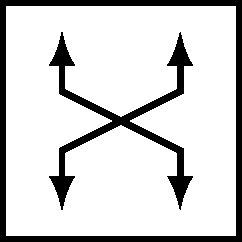
\includegraphics[width=0.9cm,alt={switch}]{../common/fig-switch.pdf}
}
\providecommand{\bigswitch}{%
    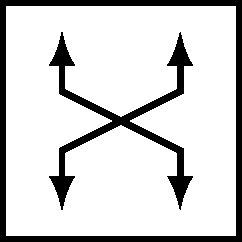
\includegraphics[width=1.4cm,alt={switch}]{../common/fig-switch.pdf}
}
\providecommand{\router}{%
    
\includegraphics[width=0.9cm,alt={router}]{../common/fig-router.pdf}
}



\begin{frame}{exercise}
\myalttext{
\begin{tikzpicture}
\tikzset{
    connect one/.style={draw,very thick,-Latex},
    connect/.style={draw,very thick,Latex-Latex},
    computer/.style={inner sep=0mm,outer sep=0mm,execute at begin node={\computer}},
    switch/.style={inner sep=0mm,outer sep=0mm,execute at begin node={\switch}},
    big switch/.style={inner sep=0mm,outer sep=0mm,execute at begin node={\bigswitch}},
    packet/.style={minimum width=.4cm,minimum height=0.2cm,inner sep=0mm,outer sep=0mm,draw},
    packet lg/.style={minimum width=.6cm,minimum height=0.2cm,inner sep=0mm,outer sep=0mm,draw},
    c1c2/.style={fill=violet!40,draw=black,thin,slidealt=<2>{thick,draw=red}},
}
\node[computer,label={center:A}] (A) at (0, 0) {};
\node[computer,label={center:B}] (B) at (5, -2) {};
\node[computer,label={center:C}] (C) at (10, 0) {};
\node[switch,label={south:S1}] (S1) at (3, 0) {};
\node[switch,label={south:S2}] (S2) at (5, 0) {};
\node[switch,label={south:S3}] (S3) at (7, 0) {};
\draw[connect] (A) -- (S1);
\draw[connect] (S1) -- (S2);
\draw[connect] (B) -- (S2);
\draw[connect] (S2) -- (S3);
\draw[connect] (S3) -- (C);
\end{tikzpicture}
}{A <-> S1 <-> S2 <-> {B, S3 <-> C}}
\begin{itemize}
\item suppose A, B, C all sending to each other (all 6 pairs).
\item where does multiplexing/demultiplexing happen?
\item where are packet drops likely?
\end{itemize}
\end{frame}
